\section{lemma9}
\begin{lemma}
\end{lemma}

Suppose we have a Riemann sphere $C$ and a diagram $(C,\iota,\xi)$ and a regular cell complex refinement $\overline{(C,\iota,\xi)}$ and a sheaf $\mathfrak{F}$ singular supported on it such that when restricted to a small disk $D\subset C$ the refinement is as the following figure where two dimensional strata are labeled :


\begin{figure}[H] % Optional: [h] means here, [t] for top, [b] for bottom, [p] for page of floats
    \centering
    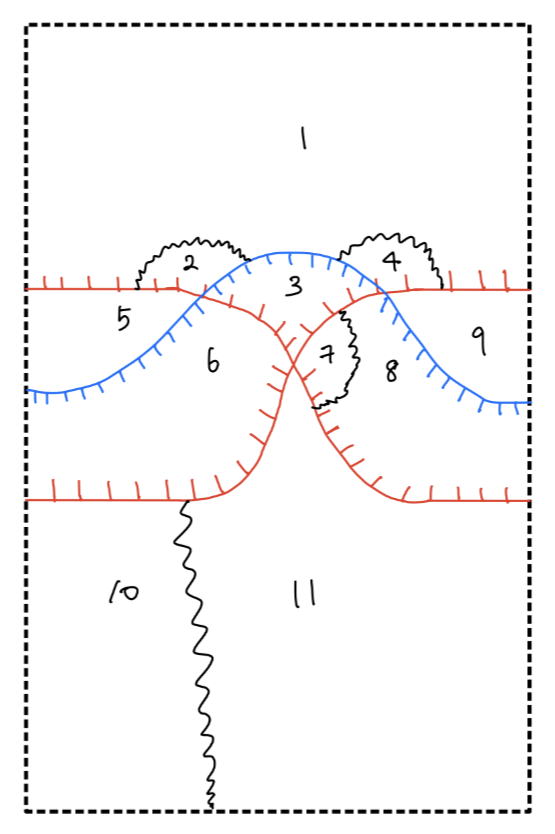
\includegraphics[scale=0.95]{diagrams/lemma9/1.png} % Adjust the width as needed
    \caption{Your caption here}
    \label{fig:your-label}
\end{figure}

Stalks :\\

- 1 : $0$\\
- 2 : $\mathbb{C}\xrightarrow{\times a}\mathbb{C}$\\
- 3 : $\mathbb{C}[-1]$\\
- 4 : $\mathbb{C}\xrightarrow{\times b}\mathbb{C}$\\
- 5 : $\mathbb{C}$\\
- 6 : $0$\\
- 7 : $\mathbb{C}\xrightarrow{\times c}\mathbb{C}$\\
- 8 : $0$\\
- 9 : $\mathbb{C}$\\
- 10 : $\mathbb{C}$\\
- 11 : $\mathbb{C}$\\

Generization maps : \\

I won't write down the zero maps.\\
- 2$\rightarrow$5 : 
\begin{tikzcd}
\mathbb{C} \arrow[r,]     & 0  \\
\mathbb{C} \arrow[r,"id"]\arrow[u,"\times a"] & \mathbb{C} \arrow[u,]
\end{tikzcd}
\\
- 3$\rightarrow$2 : 
\begin{tikzcd}
\mathbb{C} \arrow[r,"id"]     & \mathbb{C}  \\
0 \arrow[r,]\arrow[u,] & \mathbb{C} \arrow[u,"\times a"]
\end{tikzcd}
\\
- 3$\rightarrow$4 : 
\begin{tikzcd}
\mathbb{C} \arrow[r,"id"]     & \mathbb{C}  \\
0 \arrow[r,]\arrow[u,] & \mathbb{C} \arrow[u,"\times b"]
\end{tikzcd}
\\
- 4$\rightarrow$9 : 
\begin{tikzcd}
\mathbb{C} \arrow[r,]     & 0  \\
\mathbb{C} \arrow[r,"id"]\arrow[u,"\times b"] & \mathbb{C} \arrow[u,]
\end{tikzcd}
\\
- 3$\rightarrow$7 : 
\begin{tikzcd}
\mathbb{C} \arrow[r,"id"]     & \mathbb{C}  \\
0 \arrow[r,]\arrow[u,] & \mathbb{C} \arrow[u,"\times c"]
\end{tikzcd}
\\
- 7$\rightarrow$11 : 
\begin{tikzcd}
\mathbb{C} \arrow[r,]     & 0  \\
\mathbb{C} \arrow[r,"id"]\arrow[u,"\times c"] & \mathbb{C} \arrow[u,]
\end{tikzcd}
\\
- 10$\rightarrow$11 : $\mathbb{C}\xrightarrow{\times d}\mathbb{C}$\\

Now we will define isotopy starting from the above sheaf $\mathfrak{F}$ to the final sheaf $\mathfrak{F}'$. This will be called $isotopy_9$. The following figure is the sheaf $\mathfrak{F}'$ restricted to $D\subset C$.

\begin{figure}[H] % Optional: [h] means here, [t] for top, [b] for bottom, [p] for page of floats
    \centering
    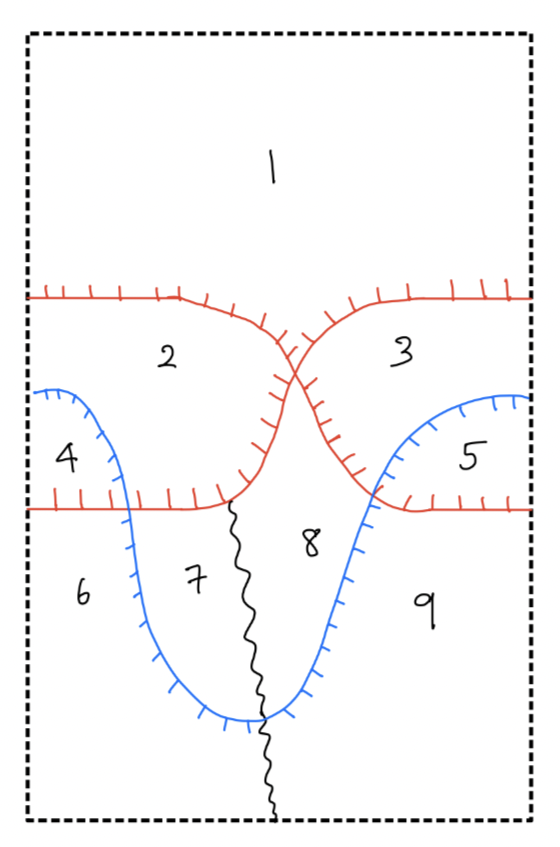
\includegraphics[scale=0.95]{diagrams/lemma9/2.png} % Adjust the width as needed
    \caption{Your caption here}
    \label{fig:your-label}
\end{figure}

Stalks : \\
- 1 : $0$\\
- 2 : $\mathfrak{C}$\\
- 3 : $\mathfrak{C}$\\
- 4 : $0$\\
- 5 : $0$\\
- 6 : $\mathfrak{C}$\\
- 7 : $\mathfrak{C}^2$\\
- 8 : $\mathfrak{C}^2$\\
- 9 : $\mathfrak{C}$\\


Generization maps :\\
-7$\rightarrow$8 : $\mathbb{C}^2\rightarrow \mathbb{C}^2$ where $e_1 \mapsto (ac^{-1},ab^{-1})^T$ and $e_2\mapsto (0,d)^T$\\
- 6 $\rightarrow$9 : $\mathbb{C}\xrightarrow{\times d}\mathbb{C}$\\
- 2 $\rightarrow$ : $\mathbb{C}\rightarrow \mathbb{C}^2$ where $e_1 \mapsto (aC^{-1},ab^{-1})^T$\\
- rest of the maps crossing red strands are $\iota_f$\\
- rest of the maps crossing blue strands are $\iota_f$\\

We define $isotopy_9$ as follows :\\
(step1) Apply $isotopy_1$ inside the disk surrounded by the purple dotted lines:
\begin{figure}[H] % Optional: [h] means here, [t] for top, [b] for bottom, [p] for page of floats
    \centering
    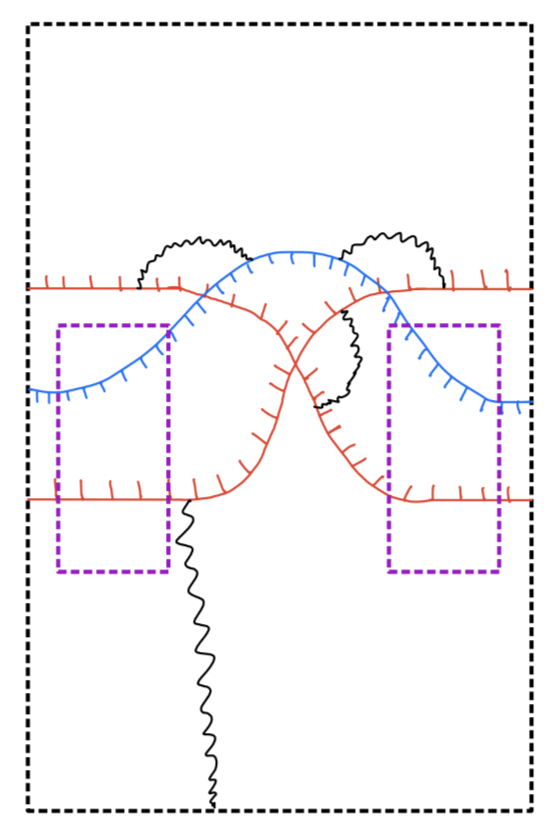
\includegraphics[scale=0.95]{diagrams/lemma9/3.png} % Adjust the width as needed
    \caption{Your caption here}
    \label{fig:your-label}
\end{figure}
We get the following diagram :
\begin{figure}[H] % Optional: [h] means here, [t] for top, [b] for bottom, [p] for page of floats
    \centering
    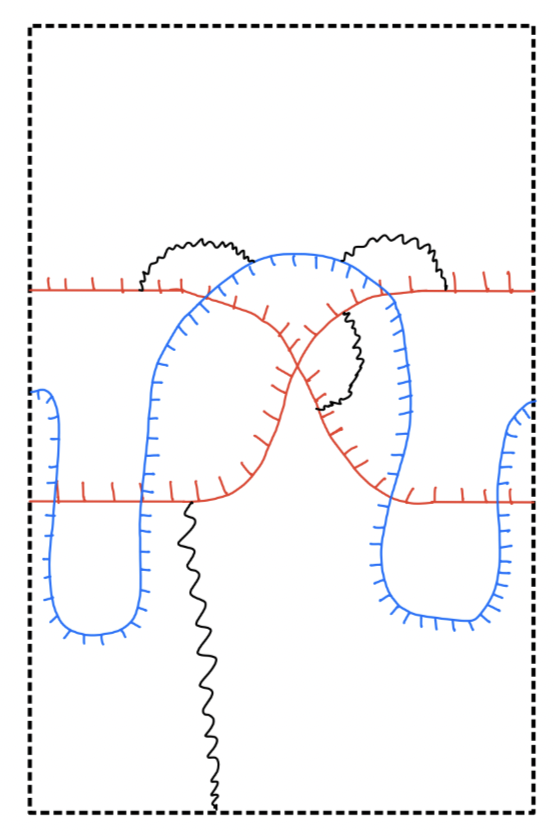
\includegraphics[scale=0.95]{diagrams/lemma9/4.png} % Adjust the width as needed
    \caption{Your caption here}
    \label{fig:your-label}
\end{figure}

(step2) Apply $isotopy_4$ on the disk surrounded by purple dotted line:
\begin{figure}[H] % Optional: [h] means here, [t] for top, [b] for bottom, [p] for page of floats
    \centering
    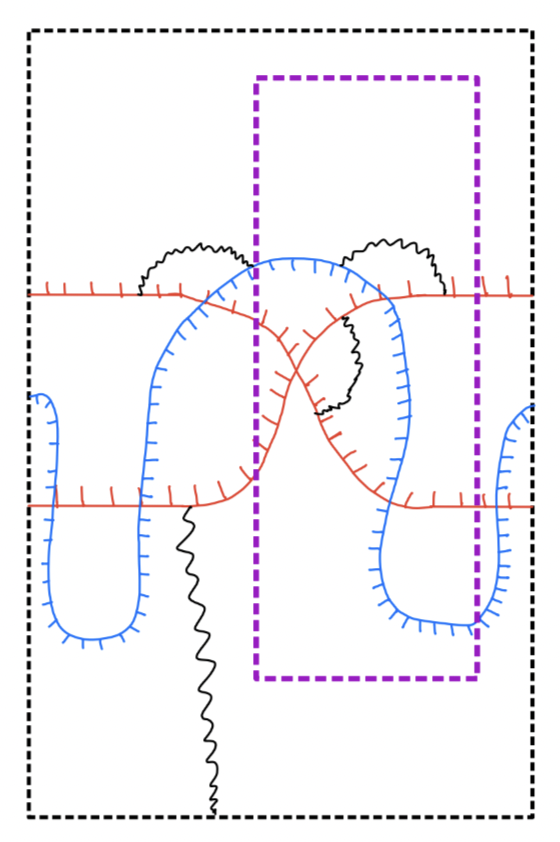
\includegraphics[scale=0.95]{diagrams/lemma9/5.png} % Adjust the width as needed
    \caption{Your caption here}
    \label{fig:your-label}
\end{figure}

We get the following diagram :
\begin{figure}[H] % Optional: [h] means here, [t] for top, [b] for bottom, [p] for page of floats
    \centering
    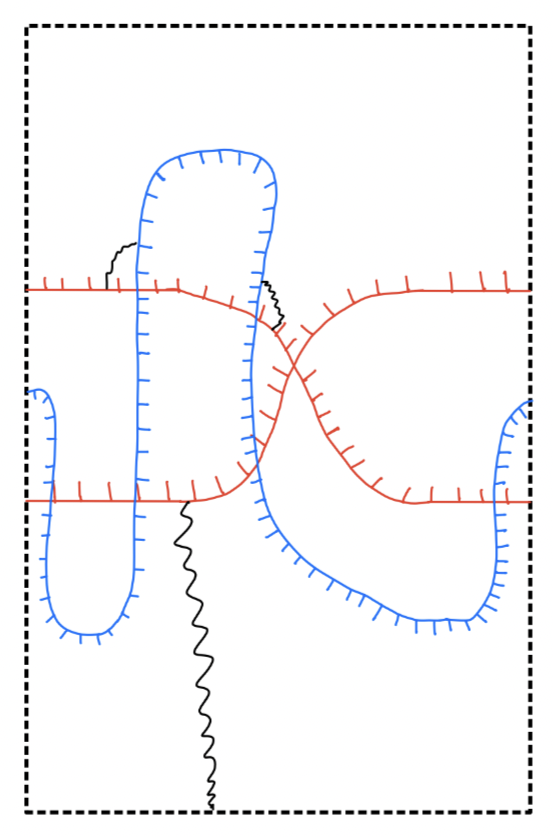
\includegraphics[scale=0.95]{diagrams/lemma9/6.png} % Adjust the width as needed
    \caption{Your caption here}
    \label{fig:your-label}
\end{figure}

(step3) Apply $isotopy_8$ on the disk surrounded by purple dotted line:
\begin{figure}[H] % Optional: [h] means here, [t] for top, [b] for bottom, [p] for page of floats
    \centering
    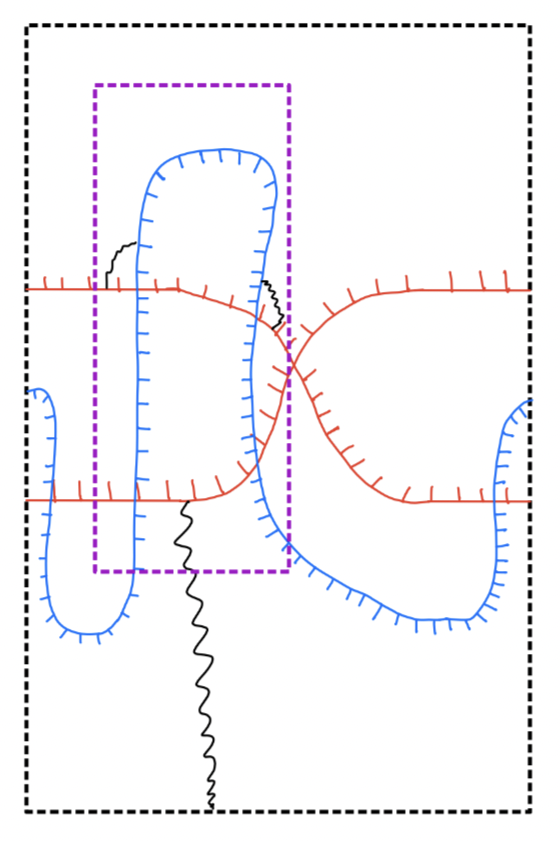
\includegraphics[scale=0.95]{diagrams/lemma9/7.png} % Adjust the width as needed
    \caption{Your caption here}
    \label{fig:your-label}
\end{figure}

we get the following diagram :
\begin{figure}[H] % Optional: [h] means here, [t] for top, [b] for bottom, [p] for page of floats
    \centering
    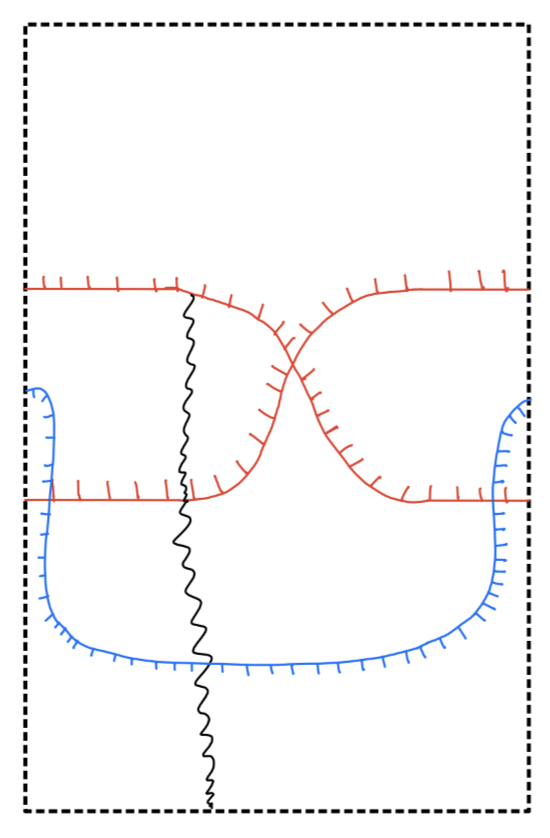
\includegraphics[scale=0.95]{diagrams/lemma9/8.png} % Adjust the width as needed
    \caption{Your caption here}
    \label{fig:your-label}
\end{figure}

(step4) we can change the basis of the stalk at the region marked with purple star so that the generization map corresponding to the squiggly line next to the purple star is the identity map:

\begin{figure}[H] % Optional: [h] means here, [t] for top, [b] for bottom, [p] for page of floats
    \centering
    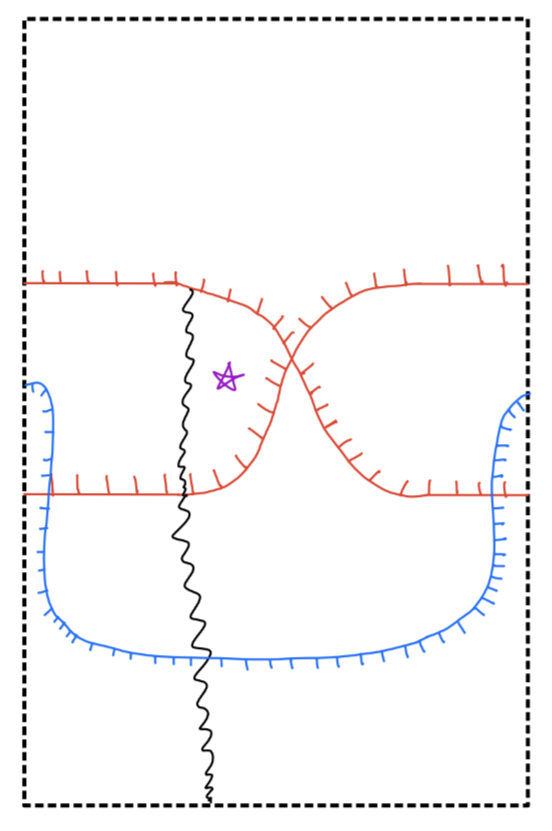
\includegraphics[scale=0.95]{diagrams/lemma9/9.png} % Adjust the width as needed
    \caption{Your caption here}
    \label{fig:your-label}
\end{figure}

Now the sheaf could be thought of as a sheaf singular supported on the below diagram:
\begin{figure}[H] % Optional: [h] means here, [t] for top, [b] for bottom, [p] for page of floats
    \centering
    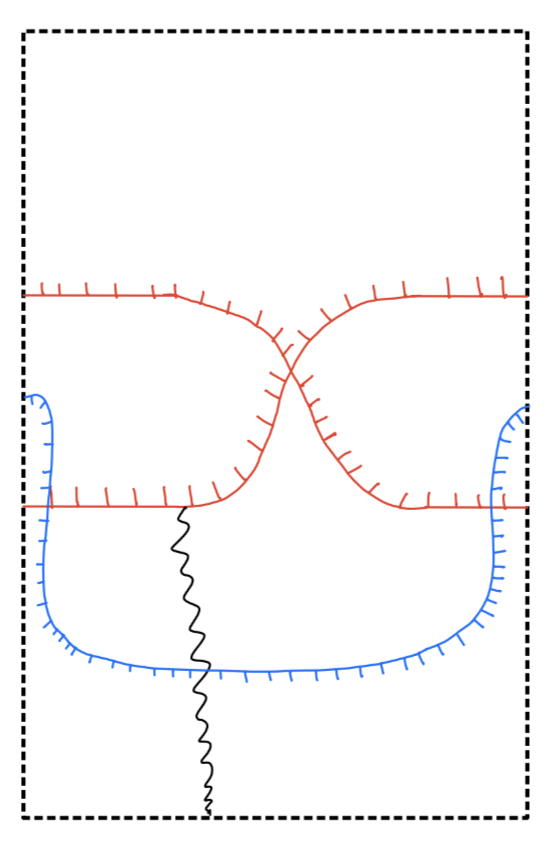
\includegraphics[scale=0.95]{diagrams/lemma9/10.png} % Adjust the width as needed
    \caption{Your caption here}
    \label{fig:your-label}
\end{figure}

and that sheaf is $\mathfrak{F}'$.\\
(proof) By Lemma1, after (step1) we get the following sheaf